\chapter{First Chapter - probably ``Introduction''}
\label{chap:chap1}





\section{Referencing} 
Whenever you refer to another's ideas or findings you should include a reference. This will allow the reader to 
locate and refer to the original source in the event of wishing to find out more information about a particular 
topic. Please note that references do not allow you to copy sections of work that are not your own. 

There are a number of conventions for citing references. You should follow the one referred to as ``Harvard'', described in great detail in the University's guide 

\verb|http://libguides.mmu.ac.uk/refguide/mmuharvard|.

The citation should be given name and a year, as in the case this case: \textcite{frith-2012}. This name form is easier to work with than others and gives some visual clue to the reference. When naming authors, use their surname only; do not use their personal names, titles or initials unless it is necessary to distinguish two people with the same surname. If there are two authors of a paper, use both their surnames to identify it \parencite{ryoo-matthies-2013}. For three or more, give the name of the first author and the words ``et al'' \parencite{chen-j-k-2015}. It is not normal to state where the authors work; this is an attempt by journalists to give credibility their statements and is not appropriate in scientific writing where we are concentrating on the content of the work.


\section{Figures and Tables}
A figure caption should appear below each figure, and a table caption should appear below each table. Insert figures 
and tables after they are cited in the text; make sure that you cite them all. The figure or table, together with the caption (which should give the number of the figure or table), should be centred and referred to within the text as ``Figure~\ref{fig:fig1} shows...'' or ``...as shown in Table~\ref{tab:tab1}''. There should be a blank line 
above and below each figure or table. 

\begin{figure}[htb]
\centering
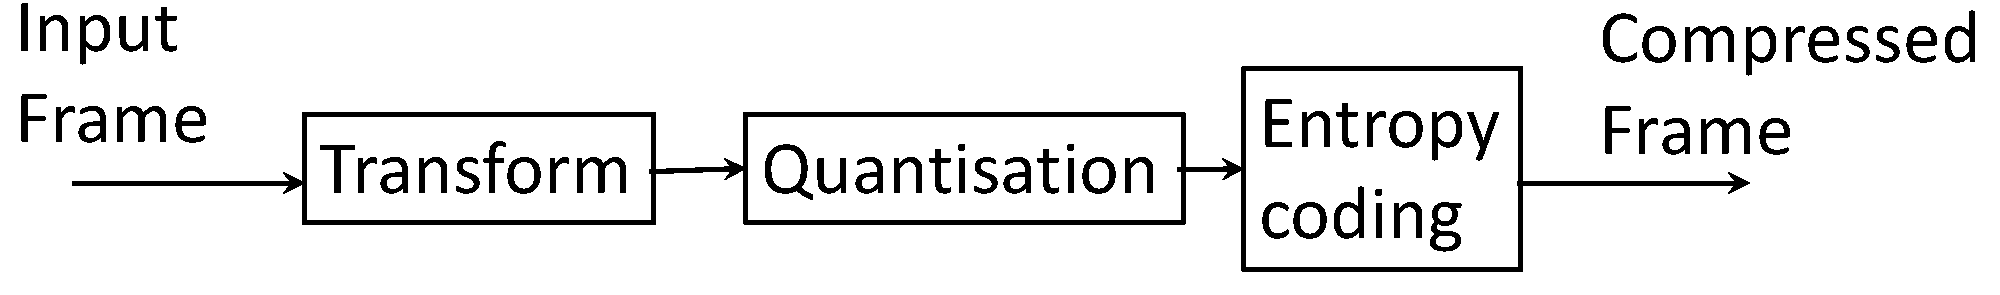
\includegraphics[width = 0.9\columnwidth]{style_guide_fig1.pdf}
\caption{Transform coding.}
\label{fig:fig1}
\end{figure}

\begin{table}[htb]
\centering
\begin{tabular}{|l|l|}
\hline
\textbf{Number} &  \textbf{Measurement} \\
\hline 
M0 & Difference in Y values \\
\hline
M1 & Maximum of TI \\
\hline 
M2 & RMS of TI \\
\hline 
M3 &  Range of TI values \\
\hline
M4 & RMS of SI \\
\hline
\end{tabular}
\caption{Quality measurements used by CQA}
\label{tab:tab1}
\end{table}

If preparing your report on Word, use its caption handling facility to enter figure and table headings. This will allow you to auto-number the 
headings and also to generate a List of Figures and a List of Tables at the beginning of your report. 

\section{Equations} 
Number equations consecutively within each chapter (e.g. the first equation in Chapter 1 should be numbered 
(1.1), the first equation in Chapter 2 should be numbered (2.1) etc.). Equation numbers, within parentheses, 
should be positioned flush right as in (\ref{equ:eqn1}). The equation should be centred and included in the sentence within your text which brackets it. There should be a blank line above and below each equation. 

The following is an example of the correct use and formatting of an equation:

\begin{quote}
Using the root mean square error,
\begin{equation}
RMSE = \sqrt{\frac{1}{N} \sum_{i=1}^{N}(x_i - m_i)^2},
\label{equ:eqn1}
\end{equation}
as a measure of accuracy, where $x_i$ and $m_i$ are respectively the $i$-th elements of the observation and reference,....
\end{quote}